% Set up the document class [paper size, font size]{class}
\documentclass[oneside,letterpaper,12pt]{article}
%%% Use American Meteorological Society Citation style
\usepackage{natbib}
\bibliographystyle{ametsoc2014}
\bibpunct{(}{)}{;}{a}{}{,}
\usepackage{proposal}

% Add nomenclature
%%%%%%%%%%%%%%%%%%%%%%%%%%%%%%%%%%%%%%%%%%%%%%%%%%%%
%%% Set up acronyms for paper
%%%%%%%%%%%%%%%%%%%%%%%%%%%%%%%%%%%%%%%%%%%%%%%%%%%%
\DeclareAcronym{OLR}{
	short = OLR,
	long  = outgoing longwave radiation
}
\DeclareAcronym{ITCZ}{
	short = ITCZ,
	long  = Intertropical Convergence Zone
}
\DeclareAcronym{SPCZ}{
	short = SPCZ,
	long  = South Pacific convergence zone
}
\DeclareAcronym{TRMM}{
	short = TRMM,
	long  = Tropical Rainfall Measuring Mission
}
\DeclareAcronym{TMI}{
	short = TMI,
	long  = \ac{TRMM} Microwave Imager
}
\DeclareAcronym{PR}{
	short = PR,
	long  = \ac{TRMM} Precipitation Radar
}
\DeclareAcronym{MERRA}{
	short = MERRA,
	long  = Modern-Era Retrospective Analysis for Research and Applications
}
\DeclareAcronym{ECMWF}{
	short = ECMWF,
	long  = European Centre for Medium-Range Weather Forecasts
}
\DeclareAcronym{ERA-Interim}{
	short = ERA-Interim,
	long  = \ac{ECMWF} Reanalysis Interim
}
\DeclareAcronym{ERAI}{
	short = ERA-Interim,
	long  = \ac{ECMWF} Reanalysis Interim
}
\DeclareAcronym{ERA5}{
	short = ERA5,
	long  = fifth generation of \ac{ECMWF} atmospheric reanalysis
}
\DeclareAcronym{ERA40}{
	short = ERA40,
	long  = \ac{ECMWF} 40-year Reanalysis
}
\DeclareAcronym{GCM}{
	short = GCM,
	long  = general circulation model
}
\DeclareAcronym{CGCM}{
	short = CGCM,
	long  = coupled general circulation model
}
\DeclareAcronym{AGCM}{
	short = AGCM,
	long  = atmospheric general circulation model
}
\DeclareAcronym{GPCP}{
	short = GPCP,
	long  = Global Precipitation Climatology Project
}
\DeclareAcronym{ISCCP}{
	short = ISCCP,
	long  = International Satellite Cloud Climatology Project
}
\DeclareAcronym{CMIP5}{
	short = CMIP5,
	long  = Coupled Model Intercomparison Project Phase 5
}
\DeclareAcronym{QTCM}{
	short = QTCM,
	long  = quasi-equilibrium tropical circulation model
}
\DeclareAcronym{JJA}{
	short = JJA,
	long  = June-August
}
\DeclareAcronym{CAM}{
	short = CAM,
	long  = Community Atmospheric Model
}
\DeclareAcronym{RSS}{
	short = RSS,
	long  = Remote Sensing Systems
}
\DeclareAcronym{RR}{
	short = RR,
	long  = rain rate
}
\DeclareAcronym{PCT}{
	short = PCT,
	long  = polarization corrected temperature
}
\DeclareAcronym{PF}{
	short = PF,
	long  = precipitation feature
}
\DeclareAcronym{RPF}{
	short = RPF,
	long  = radar precipitation feature
}
\DeclareAcronym{MEI}{
	short = MEI,
	long  = Multivariate ENSO Index
}
\DeclareAcronym{HRC}{
	short = HRC,
	long  = highly reflective cloud
}
\DeclareAcronym{MRF}{
	short = MRF,
	long  = Markov random field
}
\DeclareAcronym{TPW}{
	short = TPW,
	long  = total precipitable water
}
\DeclareAcronym{ENSO}{
	short = ENSO,
	long  = El Ni\~{n}o Southern Oscillation
}
\DeclareAcronym{CCKW}{
	short = CCKW,
	long  = convectively-coupled Kelvin wave,
	foreign-plural = {}
}
\DeclareAcronym{SST}{
	short = SST,
	long  = sea surface temperature
}
\DeclareAcronym{MODIS}{
	short = MODIS,
	long  = Moderate Resolution Imaging Spectroradiometer
}
\DeclareAcronym{MERRA2}{
	short = MERRA-2,
	long  = {Modern-Era Retrospective analysis for Research and Applications, Version 2}
}
\DeclareAcronym{CWV}{
	short = CWV,
	long  = columnar water vapor
}


%%%%%%%%%%%%%%%%%%%%%%%%%%%%%%%%%%%%%%%%%%%%%%%%%%%%
%%% Define author first and last name
%%% If you want a middle name/initial then add to first name
%%%%%%%%%%%%%%%%%%%%%%%%%%%%%%%%%%%%%%%%%%%%%%%%%%%%
\newcommand{\firstname}{Aggie D.}
\newcommand{\lastname}{Student}

%%%%%%%%%%%%%%%%%%%%%%%%%%%%%%%%%%%%%%%%%%%%%%%%%%%%
%%% Set up the type of graphics to use
%%%%%%%%%%%%%%%%%%%%%%%%%%%%%%%%%%%%%%%%%%%%%%%%%%%%
%\DeclareGraphicsExtensions{.eps}
%\graphicspath{{/Volumes/ExtraHDD/Plots/PostScript/Thesis_Proposal/}}

\DeclareGraphicsExtensions{.png}

%%%%%%%%%%%%%%%%%%%%%%%%%%%%%%%%%%%%%%%%
%
%	 MAIN TEXT	MAIN TEXT		MAIN TEXT		MAIN TEXT		MAIN TEXT
%
%%%%%%%%%%%%%%%%%%%%%%%%%%%%%%%%%%%%%%%%
\begin{document} 

\title{Very good proposal title for my research} % set title for document

\doublespacing

%%%%%%%%%%%%%%%%%%%%%%%
%%% Introduction
\section{Introduction}

This is the introduction of the document.
You should provied backround information settin up your research and why it is important.
If you are using BibTeX for references, you can use the various commands to references papers.
For this example, the Americal Meterorlogical Society reference style is used.
That means we can cite \citet{Masunaga_etal:2005} and why their research is great.
We can also talk about how their results bring more context to existing theories \citep{Henderson_etal:2018}.

If you have set up the nomenclature file, you can also use acronyms very easily, such as \ac{ITCZ}.
This package will keep track of if you have used an acronym, giving the full definition the first time and the short version everytime after, such as \ac{ITCZ}.

%%%%%%
%%% Objectives
\section{Research Objectives}
This is a good section to really outline your objective and spell out your hypotheses.
You can use a table to such as the one below to itemize them:

\begin{enumerate}[label=H\arabic*.]\bfseries
   \item Gravity makes things fall toward the center of the Earth
   \item Every action has an equal and opposite reaction
\end{enumerate}


%%%%%%%%%%%%%%%
%%% Data
\section{Data \& Methods}
Here is where you can discuss the various datasets you will be using, giving some background to why they will be used and some limitations of the data.
These do not need to be in subsections, but it may be useful to separate them as such if there are many different datasets being used.

\subsection{ERA5}
Talk about why you are using this, advantages/disadvantages, etc.

\subsection{Preprocessing}
Any regridding, post-processing, etc. that is performed, or planned, can be discussed in this subsection.

%%%%%%%%%%%%%%%
\section*{Research section/chapter}
The following sections can talk about the various projects in your research.
It is somewhat typical for a PhD student to publish three papers, and then combine those into a dissertation.
In that case, you could have three sections here the discuss what those papers are, or are going to be, about.

If some of the work has been completed, as would probably be the case for at least the first chapter, you could include a figure illustrating key findings from the work.

\begin{figure}[!t]
	\centering
	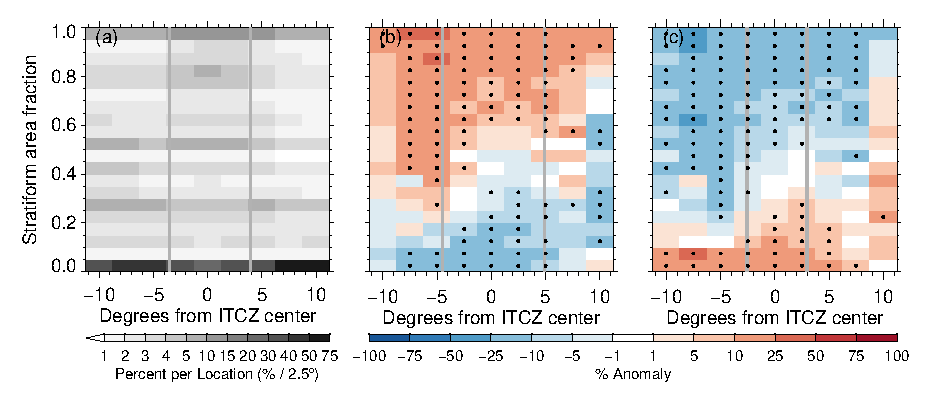
\includegraphics[width=0.9\textwidth]{./Figures/stratFrac_2d.eps}
	\caption{
		Joint histograms of PF stratiform area fraction and distance from the center of the ITCZ for (a) climatology, (b) mean of monthly percent anomalies in wide ITCZ months, and (c) mean of monthly anomalies in narrow ITCZ months.
		Distances are relative to the center of the ITCZ (positive north) and are in units of degrees.
		The vertical gray lines in all panels represent the location of the ITCZ boundaries for each data subset.
		Stippling indicates anomalies that are significantly different from zero at the 95\% level based on 10,000 random resamples with replacement.
	}
	\label{fig:stratiform2D}
\end{figure}

You can then reference figure \ref{fig:stratiform2D} as so.

%%%%%%%%%%%%%%%%%%%%%%%%
\section*{Research section/chapter 2}
Here is another part of the research and a figure for this section.

\begin{figure}[!b]
	\centering
	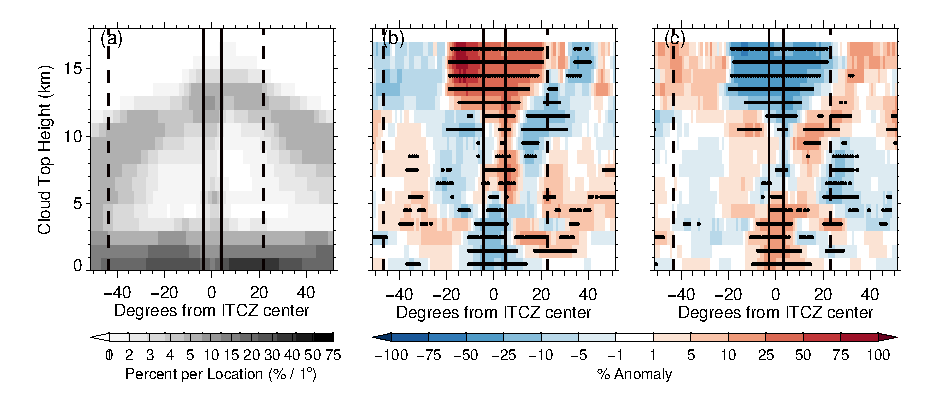
\includegraphics[width=0.9\textwidth]{./Figures/cloudHeightAqua.eps}
	\caption{
		As in Figure \ref{fig:stratiform2D}, but for MODIS cloud top height.
		The solid and dashed vertical black lines in all panels represent the location of the ITCZ and Hadley cell boundaries, respectively, for each data subset.
		Stippling indicates anomalies that are significantly different from zero at the 95\% level based on 10,000 random resamples with replacement.
	}
	\label{fig:modis}
\end{figure}

%%%%%%%%%%%%%%%
%%% Timeline 
\section{Timeline for completion}
A breif discussion about timeline for completetion.
Can state that first portion of work is published, second portion is submitted, and third piece is in data analysis stage.
Obviously these must be adjusted to make your current state of progress.

%%%%%%%%%%%%%%%
%%% References
\bibliography{References_Database}

\end{document}
